\documentclass[../../Thesis.tex]{subfiles}
\begin{document}
\header{Corpus}
The dataset we used for this research consists of articles published in 2017 which have been published in a journal that has, in 2017, atleast 150 publications. This results in a total dataset of $1.391.543$ articles from $3.759$ journals. Details about the corpus can be found in table~\ref{table:corpusSize}.
\begin{table}[hbt]
\begin{center}
\begin{tabular}{|l|c|c|c|}
\hline
 & Total count & Unique count & Average length \\
\hline\hline
Title words & $18.822.399$ & $939.665$ & 13,53  \\
\hline
Title tokens & $14.742.192$ & $230.805$ & 10,64 \\
\hline\hline
Abstract words & $264.653.020$ & $5.853.077$  & 190,19  \\
\hline
Abstract tokens & $171.474.473$ & $738.961$ & 123,71 \\
\hline\hline
Total words & $283.475.419$ & $6.209.769$  & 203,71 \\
\hline
Total tokens & $186.962.354$ & $763.475$ & 134,36 \\
\hline
\end{tabular}
\end{center}
\caption{Corpus size}\label{table:corpusSize}
\end{table}\\
The word occurrences follow the pattern of a pareto distribution as described by~\citet{wiegand2018word}. This distribution is visualized in figure~\ref{figure:wordTokenOccurrence}, which displays the occurrences of the first 500 tokens of the corpus.
\begin{figure}[hbt]
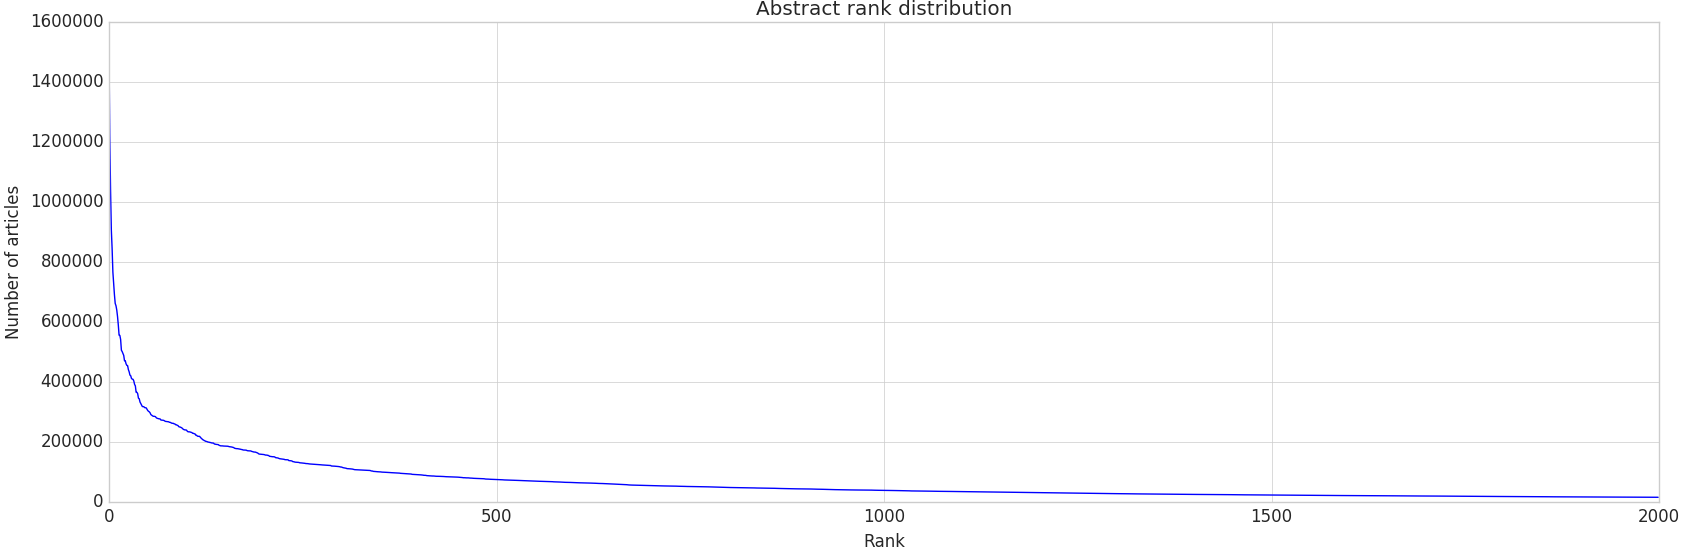
\includegraphics[width=6.5in]{Plots/word_occurrences}
\caption{Word and token occurrences}\label{figure:wordTokenOccurrence}
\end{figure}

\header{Datasets}
For this researched we used a (pre-made) tokenized dataset, which reduces the total amount of words by 34\%, from this tokenized set, we created the embeddings and the TF-IDF feature vectors.
\subheader{Tokenization}
The following steps have been applied to the words to create a tokenized set:
\begin{enumerate}
\item{Removed punctuation}
\item{Removed all non-ascii characters}
\item{Transformed all characters to lower-case}
\item{Removed stop-words, as provided by the NLTK library}
\item{Removed numbers}
\item{Stemmed all words, using the stemmer provided by the NLTK library}
\end{enumerate}
These transformations reduced our dataset by 34\%, resulting in a tokenized set of $186.962.354$ tokens.

\subheader{Embedding}
For this research we reused the word embeddings created by \citet{Truong2017Thesis}. These embeddings have a vector size of 300, which is an industry default. They have been trained on the entire Elsevier corpus, not limited to the subset we used for this research. To construct article embeddings we take the average of all normalized word embeddings for that article. Journal embeddings are constructed in the same way, we averaged all the normalized article embeddings to create the journal embeddings. We have used multiple embedding configurations for this research
\subsubheader{Default embedding}
The default embedding is created form the pre-trained word embeddings, no modifications have been applied to this set.
\subsubheader{TF-IDF embedding}
The TF-IDF weighted embedding set, referred to as TF-IDF embedding, are the default word embeddings weighted with a TF-IDF score per word.\\
The TF-IDF is calculated with a raw token count, and a smoothed inverted document frequency, calculated as follows:\\
\begin{equation}
IDF = \log_{10}(\dfrac{|A|}{|A_t|})
\end{equation}
Where $|A|$ is the total count of articles and $|A_t|$ is the count of articles containing term t.
The articles embeddings are a normalized summation of each word vector multiplied by it TF-IDF value. Since we take a sum of all words, the Term Frequency is embedded as the raw count of each word.
\subsubheader{10K TF-IDF embedding}
The 10K embedding set is generated similarity to the TF-IDF embedding, this version only uses the 10.000 most common tokens, reducing the amount of tokens it uses. This set was created to see if the limitation to 10.000 tokens reduces the amount of noise, and with that increasing the performance.
\subsubheader{5K TF-IDF embedding}
The 5K TF-IDF embedding is the TF-IDF embedding set, limited to the 5.000 most common words. This set was created to more aggressively limit the amount of tokens, and with that, cancel out more noise.
\subsubheader{1K-6K TF-IDF embedding}
The 1K-6K TF-IDF embedding is the TF-IDF embedding limited to the top 6.000 most common words, without the top 1.000 most common words. The rationale for this is that common words will occur in many articles, creating noise, by cutting of the top 1.000 and cutting of everything below 6.000 we tried to reduce the noise by filtering common words. This cut results in a set of 5.000 tokens, which allows us to compare it to the 5K TF-IDF set.

\subheader{TF-IDF}
To create the TF-IDF feature vectors, we used the TF-IDF model and a hasher from pysparks the MlLib library. The TF-IDF feature vectors are created by hashing the tokens with the hasher, which has a set hash bucket size. These hashed values are passed on to the TF-IDF model, resulting in a feature vector which vector dimensions equals the amount of hash buckets. To limit the computational and storage expenses and to reduce noise by rare words, we limit our vocabulary size.
We denote the TF-IDF configurations as follows: $vocabulary size/hashbucket size$. Furthermore, we denote 1.000 as 1K, since we deal with chosen values which can be exactly noted given this notation.
\begin{figure}
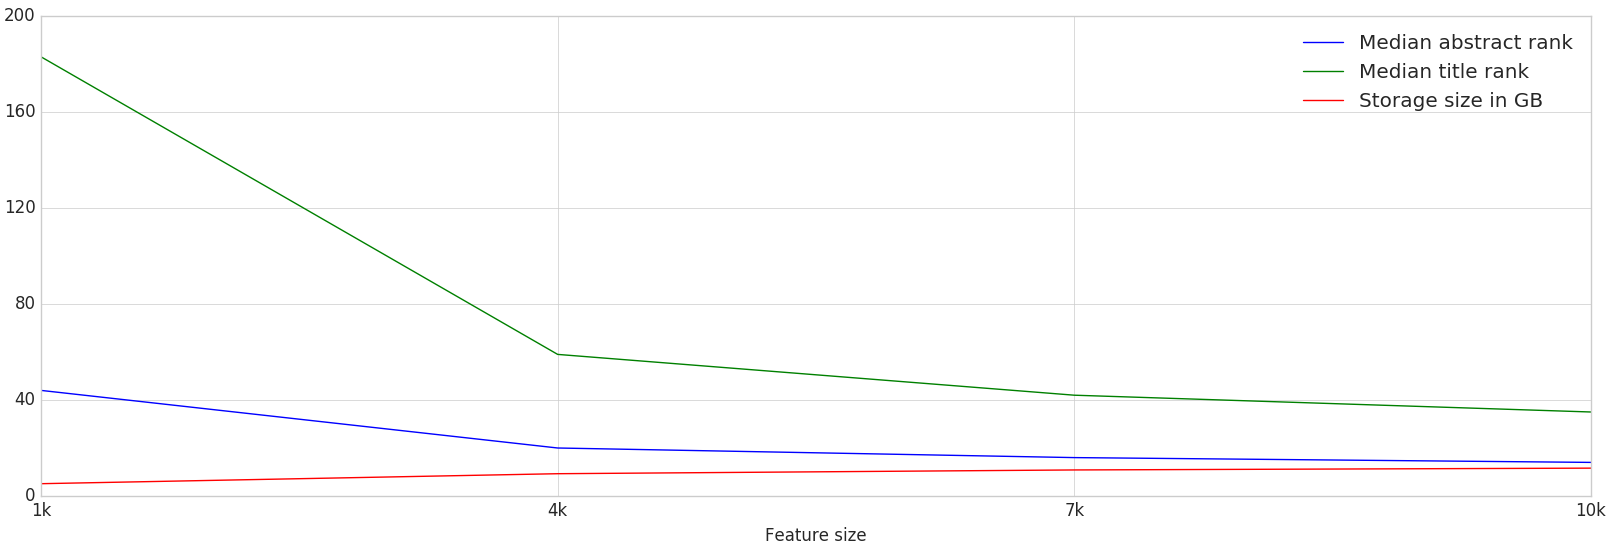
\includegraphics[width=6in]{Plots/tfidf_selection_plot}
\caption{TF-IDF performance and memory usage}\label{figure:tfidfPerformance}
\end{figure}
\FloatBarrier
Figure~\ref{figure:tfidfPerformance} shows the performance, as median rank, and storage size, in gigabyte, of the 1k/1K, 4K/4K, 7K/7K and 10K/10K TF-IDF configurations. This plot shows that, while the required storage size keeps rising, the performance on title quickly stagnates, and the performance on abstract follows too. Given this information, we have chosen to use the 10K/10K, 10K/5K and 5K/5K configurations to compare our embedding results to. The TF-IDF features are created on article level. We average the set of article embeddings to create a journal embedding. 

\header{Pipeline}
We procesessed the TF-IDF sets and the embedding sets via the same pipeline, using their common vector properties. This ensures comparable results, the pipeline is set-up as follows:
\begin{enumerate}
\item{Create training and validation set}
\item{Create journal embeddings}
\item{Categorize validation articles}
\item{Calculate performance metrics}
\end{enumerate}
  
\subheader{Create training and validation set}
We split our initial set  $80\%$ - $20\%$,. We use the $80\%$ set as the training set for the journal representations, and the $20\%$ set as the validation set for the journal representations. This split is based on a random number given to article each record, ensuring that all set have the same (random) training and validation set.
\subheader{Create journal embeddings}
From our training set we create the journal embeddings, which are created for most sets\footnote{see paragraph datasets} by averaging the article embeddings or feature vectors.
\subheader{Categorize validation articles}
To categorize the articles, we calculate the distance between the title- and abstract embedding of each article, from the validation set, to the title- and abstract embedding of each journal, during this process we keep track of:
\begin{itemize}
\item{Title-based-rank of the actual journal}
\item{Abstract-based-rank of the actual journal}
\item{Best scored journal on the abstract similarity}
\item{Best scored journal on the title similarity}
\item{Abstract similarity between the actual journal and the article}
\item{Title similarity between the actual journal and the article}
\end{itemize}
\subsubheader{Distance metrics}
To calculate the distance between to vectors, cosine similarity is commonly used. We validated the quality of cosine similarity as a distance metrics by comparing it to all other similarity matrices available in the SciPy library, which we used to calculate the distances. We calculate the similarities based on the normalized embeddings, and compared the distance metrics based on the default embedding set. Table~\ref{table:distanceMetrics} shows the results of this validation.\\
\begin{table}[hbt]
\begin{tabular}{|l|l|l|l|l|}
\hline
Metric\footnote{As defined and provided by the SciPy library} & Median title rank & Average title rank & Median abstract rank & Average abstract rank  \\
\hline
Braycurtis & 28 & 130 & 23 & 124  \\
\hline
Canberra & 33 & 148 & 26 & 133  \\
\hline
Chebyshev & 57 & 256 & 41 & 191  \\
\hline
\textit{Cityblock} & \textit{28} & \textit{130} & \textit{23} & \textit{124}  \\
\hline
\textit{Correlation} & \textit{27} & \textit{127} & \textit{23} & \textit{122}  \\
\hline
\textbf{Cosine} & \textbf{27} & \textbf{127} & \textbf{23} & \textbf{122}  \\
\hline
Dice & 1995 & 1929 & 1995 & 1929  \\
\hline
\textit{Euclidean} & \textit{27} & \textit{127} & \textit{23} & \textit{122}  \\
\hline
Hamming & 1995 & 1929 & 1995 & 1929  \\
\hline
Jaccard & 1995 & 1929 & 1995 & 1929  \\
\hline
Kulsinski & 1995 & 1929 & 1995 & 1929  \\
\hline
Mahalanobis & 136 & 544 & 75 & 449  \\
\hline
Matching & 1995 & 1929 & 1995 & 1929  \\
\hline
Rogerstanimoto & 1995 & 1929 & 1995 & 1929  \\
\hline
Russellrao & 1995 & 1929 & 1995 & 1929  \\
\hline
\textit{Seuclidean} & \textit{27} & \textit{124} & \textit{22} & \textit{115}  \\
\hline
Sokalmichener & 1995 & 1929 & 1995 & 1929  \\
\hline
Sokalsneath & 1995 & 1929 & 1995 & 1929  \\
\hline
\textit{Sqeuclidean} & \textit{27} & \textit{127} & \textit{23} & \textit{122}  \\
\hline
Yule & 1995 & 1929 & 1995 & 1929  \\
\hline
\end{tabular}
\caption{Distance metric performance for word embeddings on the categorization of academic texts}\label{table:distanceMetrics}
\end{table}
These results show high similarity between cosine-based metrics (Cosine \& Correlation) and euclidean based metrics (Euclidean, Seuclidean \& Sqeuclidean). This similarity is expected, since the cosine and euclidean distances should yield the same results on normalized sets. The results show that some enhancement on the euclidean algorithm result in slightly improved results, although not significant. Also the Cityblock metric yields results close to the Cosine metric, it has a slightly worse performance, which is also not significant. Because of this, we will use the cosine-similarity as the distance matrix, which will make our results better comparable with other work.

\subheader{Performance measurement}
We use multiple metrics to validate the performance of the embedding sets and TF-IDF sets on the categorization task. These metrics are:
\begin{enumerate}
\item{F1-score}
\item{Median \& average rank}
\item{Rank distribution}
\end{enumerate}
\subsubheader{F1-score}
We define the positive \& negative metrics as follows:\\
\begin{jumpin}
$True Positive = $ Articles that are correctly matched to the current journal\\
$False Positive = $ Articles that are incorrectly matched to other journals\\
$False Negative = $ Articles that are incorrectly matched to the current journal\\
\end{jumpin}
We used these metrics to calculate the Recall, Precision \& F1 as follows:\\
\begin{jumpin}
$Recall = \dfrac{True Positive}{True Positive + False Negative}$\vspace{0.1in}\\
$Precision = \dfrac{True Positive}{True Positive + False Positive}$\vspace{0.1in}\\
$F1 = \dfrac{2 * Precision * Recall}{Precision + Recall}$
\end{jumpin}
\subsubheader{Median \& average rank}
We use the median rank to indicate around which rank the 'standard' article would be ranked, based on its title or abstract. We do this by taking the median of the respective rank from each article. This gives us an indication of the behaviour of most articles in our validation set. This median rank (mostly) ignores the outliers, we therefore also use the average rank, which gives a more global indication, although this rank may be over-influenced by some outliers.
\subsubheader{Rank distribution}
To further analyse the ranking results, we plot the rank distribution to get an indication of the ranking-landscape.

\header{Two dimensional plot}
To create a plot, we transformed the 300-dimensional journal vectors into 2-dimensional vectors using TSNE based on pca\footnote{Principal component analysis}. These 2-dimensional vectors, representing the x \& y coordinate, can then be drawn in a plot. To visualize the preservation of journal-relatedness while converting the 300 dimensions to 2 dimension, we create groupings using k-means. These groupings are created on the 300-dimensional vectors, and are visualized in the plot using colors.
\end{document}

% RAW DATA:
% 1,391,543 articles
% 14 811 433 title tokens			230805 unique		18.822.399			939.665
% 172 150 921 abstract tokens		738961 unique		264.653.020			5.853.077
% 186 962 354 total tokens			763475 unique		283.475.419			6.209.769
% 3,759 journals

% split = 79.9509609117 - 20.0490390883

% training numbers
% 10K = percentage?}